\input{../../../../Skript_praeambel.tex}
\addbibresource{BibliographyIPSA.bib}

% !TeX spellcheck = en_US

\begin{document}
%Ben�tigte Angaben f�r die Titelseite
\title{Summary of the lecture \\ `Image Processing'\! \\ by Prof. Christian Bauckhage \\ (WiSe 2021/2022)}
%Hier Zeilenumbruch durch \\, da \newline in dieser Umgebung nicht funktioniert.
\author{Fabrice Beaumont \\ Matrikel-Nr: 2747609 \\
Rheinische Friedrich-Wilhelms-Universit�t Bonn}

%Erstellung des Titels
\maketitle
%\tableofcontents
%\listoffigures

%----------------------------------------------------------

%TODO: Improve slides:
% Lecture 03 - slide 48 - "...such that IT resembles..."




%%%%%%%%%%%%%%%%%%%%%%%%%%%%%%%%%%
%%%%% Lecture 01 - 11.10.2021 %%%%
%%%%%%%%%%%%%%%%%%%%%%%%%%%%%%%%%%

% USEFUL LINKS:
% - researchgate.net/project/P3ML-ML-Engineering-Knowledge
% - researchgate.net/project/Machine-Learning-Rhine-Ruhr-ML2R
% - www.b-it-center.de/students/teaching-material/p3ml

% Recommended books:
% - R. Gonzales and R.E. Woods; 'Digital Image Processing'; Prentice Hall, 3rd edition, 2007
% - B. J�hne; 'Digital Image Processing'; Springer, 6th edition, 2005
% - M. Sonka et al.; 'Image Processing, Analysis and Machine Vision'; Cengage, 3rd edition, 2007
% - D.A. Forsyth and J. Ponce; 'Computer Vision: A Modern Approach'; Prentice Hall, 2002
% - R. Hartley and A. Zisserman; 'Multiple View Geometry in Computer Vision'; Cambridge University Press, 2nd edition, 2004
% - G. Wolberg; 'Digital Image Warping'; IEEE Comp. Soc. Press, 1990

\setcounter{chapter}{1}
\chapter{Digital Photography}
%TODO: ANKI bis hier

\section{Image acquisition and digital photography}

(Digital) photography is the practice of visualizing, recording and storing light.

\begin{Definition}[Light]{def:Light}
	\textbf{Light} can be described as both\begin{itemize}
		\item as electromagnetic radiation where energy propagates in form of electromagnetic waves and 
		\item as a particle or quantum phenomenon where photons carry the electromagnetic force.
	\end{itemize}

	Light has a constant \textit{speed} of $c := \SI{299792458}{\sfrac{m}{s}}$. Light can have different \textit{frequency} $\nu$ ($[\SI{}{\per\second}]$) and \textit{wavelength} $\lambda$ ($[\SI{}{\metre}]$), but these properties are reciprocal:
	\begin{equation}
		c = \nu \lambda		\qquad \Big[\frac{\SI{}{\metre}}{\SI{}{\second}}\Big]
	\end{equation}
	
	The \textit{energy} $E$ of light is defined as
	\begin{equation}
		E = h\nu = h\frac{c}{\lambda}		\qquad \Big[\SI{}{\joule}\Big]
	\end{equation}
	where $h = 6.6260689633\times10^{-34} [\SI{}{\joule\second}]$ is the \textbf{Planck's constant}.
\end{Definition}

From these definitions we can derive the relation that light with a high frequency and small wavelength carries more energy.

\begin{figure}[H]
	\centering
	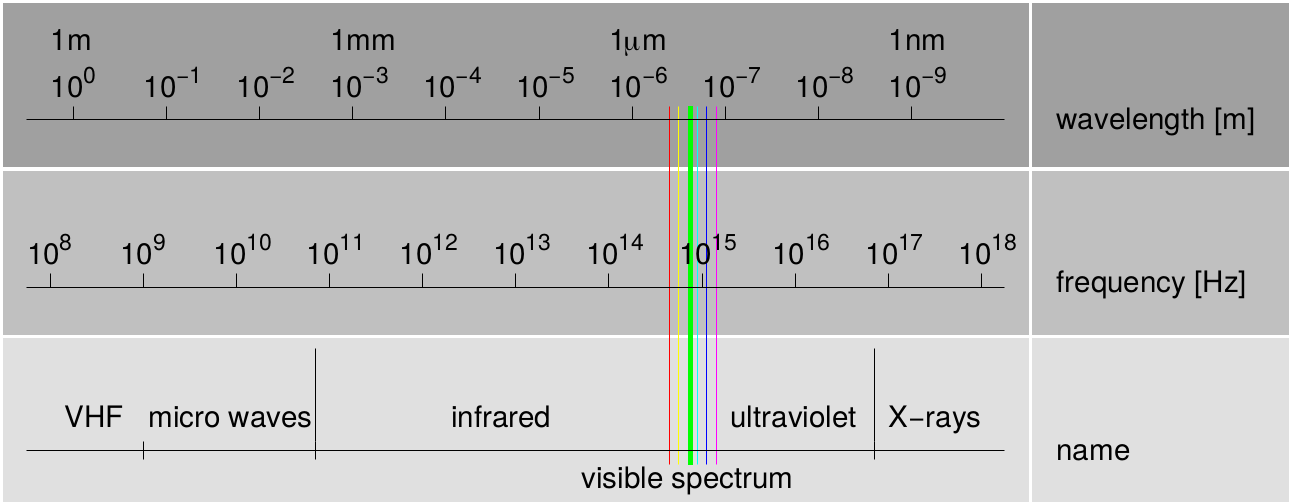
\includegraphics[width=0.8\linewidth]{images/ElectromagneticSpectrumOverview}
	\caption{Overview over the electromagnetic spectrum.}
	\label{fig:electromagneticspectrumoverview}
\end{figure}

There are three ways to visualize light. It can be:\begin{itemize}
	\item \textbf{reflected} (e.g. photographic images or scanned images),
	\item \textbf{absorbed} (e.g. X-ray images) or
	\item \textbf{emitted} (infrared images).
\end{itemize}

There are several ways to record light. Digital (color-)photography relies on CCD cameras. CCD stands for \textbf{charged-coupled device} and describes a semiconductor device consisting of photosensitive elements. Modern consumer cameras have at least $1600\times 1200$ such elements.

Rays of light incident on the camera lens hit the CCD matrix. These photons generate a charge on the CCD elements by freeing electrons. The more light there is, the more electrons are freed. Depending on the camera quality, a single CCD element stores \num[group-separator={,}]{100000} to \num[group-separator={,}]{350000} electrons before saturating. An electric field gathers electrons into packets which are read and quantized into intensity levels. Thus every CCD element records a value of light intensity.

Since the amount of represented intensity levels relates to the needed memory bits per CCD, and since the perception of the human visual system is limited in this regard, typical images typically only store $2^8 = 256$ intensity levels (one byte) per color channel (intensity quantization).

\begin{Definition}[Intensity image]{def:IntensityImage}
	\textbf{Intensity images} (\textbf{grayscale images}) do not contain color information and only display recorded light intensity (luminescence) per pixel in terms of shades of gray.
\end{Definition}

\begin{Definition}[Color image]{def:Color images}
	\textbf{Color images} do contain color information and split the recorded light into basic colors (commonly red, green and blue) from which the appropriate colors can be reconstructed on a display device later. To split the light one can use either a \textbf{trichroic prism} and record each basic color in a separate CCD array, or superimpose a mosaic of color filters (\textbf{Bayer filter}) over a single CCD array. Since the latter technique uses three times less CCD elements it is much cheaper (but also less accurate).
\end{Definition}

\begin{figure}[H]
	\centering
	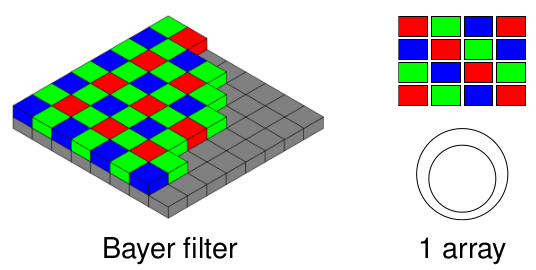
\includegraphics[width=0.45\linewidth]{images/BayerFilter}
	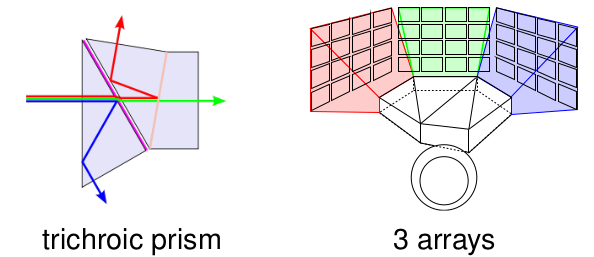
\includegraphics[width=0.45\linewidth]{images/TrichroicPrism}
	\caption{Two techniques of CCD cameras to split recoreded light into three basic colors.}
	\label{fig:ColorImagesCCDTechniques}
\end{figure}

There are several problems with the CCD technology:\begin{itemize}
	\item \textbf{Geometric distortions}. CCD elements are typically not perfectly square. This may necessitate computational correction to compensate for geometric distortions.
	\item \textbf{Blooming}. Overexposure may free to many electrons, which may overflow to neighboring elements and cause highlight effects.
	\item \textbf{Dark noise}. CCD sensors are sensitive to parts of the invisible electromagnetic spectrum (UV or IR radiation) and may thus record invisible apparitions.
\end{itemize}

There are numerous file formats for storing digital images. But these can be separated into two main types of image file formats:\begin{itemize}
	\item vector graphics formats (e.g. SVG, FIG) and
	\item pixmaps (bitmap, raster graphics; e.g. JPG, GIF, PNG, TIFF).
\end{itemize}

\begin{Definition}[PPM format]{def:PPMFormat}
	The \textbf{PPM} (\textbf{portable pixmap}) \textbf{format} stores image data in the following way:\\
	The first four lines in the file format contain:\begin{enumerate}
		\item a magic number (indicating ASCII [P1, P2, P3] or binary [P4, P5, P6] format),
		\item comments,
		\item image width and image height and
		\item the maximum color value (which is the same for all color channels).
	\end{enumerate}
	After these lines, the image data is stored in red-green-blue-triples of hexadecimal values.
\end{Definition}

\begin{figure}[H]
	\centering
	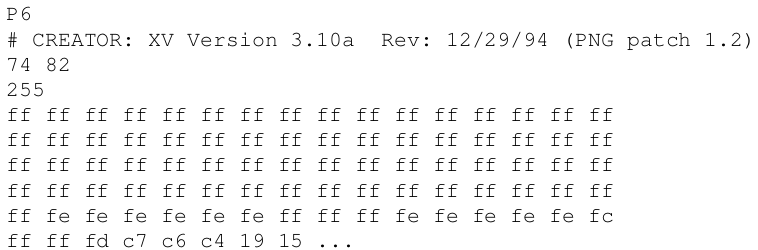
\includegraphics[width=0.8\linewidth]{images/PPMExample}
	\caption{Example header of a PPM file.}
	\label{fig:ppmexample}
\end{figure}

Keep in mind, that there are many different ways of image compression. In general these annihilate information and thus reduce memory requirements.

\section{Representations of digital images}

As explained, a digital image represents digitized and quantized information. The basic element of digital images are called \textbf{pixels} (picture elements), which are (commonly) arranged on a rectangular grid called a \textbf{pixmap}. The \textbf{resolution} of a digital image is expressed in terms of width times height of its pixmap.

Digital images often have an aspect ratio of 4:3 (e.g. $1024\times 768$) or 16:9 (e.g. $1920\times 1080$).

In memory, intensity images are stored in a single pixmap. Color images are stored in three to four pixmaps. One per color channel and a possible $\alpha$-layer. Accordingly, these images can be stored in two-, three- or four-dimensional arrays. Rows and columns of a pixel array are counted from zero and the pixel $p_{0,0}$ is located in the \textit{upper left corner} of the pixel array.

\begin{Definition}[4-Neighborhood]{def:4Neighborhood}
	The \textbf{4-neighborhood} of a pixel is the set of the two vertically and the two horizontally adjacent pixels.
\end{Definition}

\begin{Definition}[8-Neighborhood]{def:8Neighborhood}
	The \textbf{8-neighborhood} of a pixel is the set of the 4-neighborhood and the four diagonally adjacent pixels.
\end{Definition}

\begin{figure}[H]
	\centering
	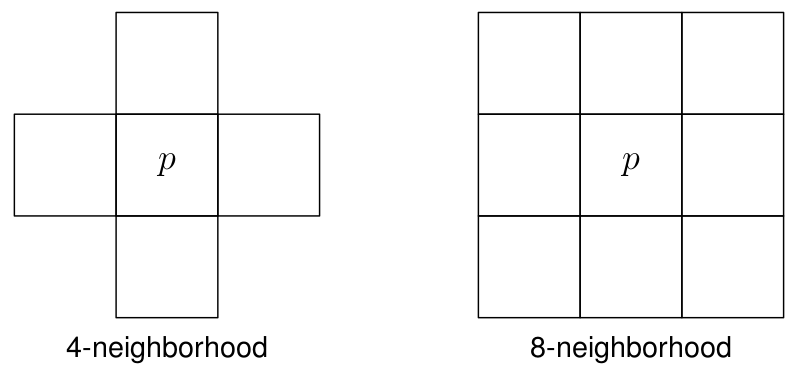
\includegraphics[width=0.7\linewidth]{images/FourAndEightNeighborhood}
	\caption{}
	\label{fig:fourandeightneighborhood}
\end{figure}

Note that the Euclidean distance yields different distances between the pixels in the 8-neighborhood. It is possible to use another metric or another arrangement of the pixelmap (e.g. a hexagonal-grid), but the technically simplest approach with respect to computer memory is the default rectangular grid.

\subsection{Images as functions}

In a digital intensity image, array coordinates $[i,j] \in \{0,\dots,M-1\}\times\{0,\dots,N-1\}$ are mapped to intensity values $p_{i,j}\in \{0,\dots,L-1\}$. Thus one may think of such an image as a \textbf{bi-variate discrete function with finite domain} $f:\IR_+^2\to \IR_+$.

Since the pixels are enumerated from the upper left corner, mapping the planar points $[x_j,y_i]$ to the images array coordinates $[i,j]$ is done as 
\begin{equation}
	[x_i,y_j] \leftrightarrow [j,M-1-i]
\end{equation}

Also, we assume that the two-dimensional point at which an image function is defined are equally spaced. More precise, the horizontal and vertical distances between neighboring point amounts to one:
\begin{equation}
\begin{aligned}
	\delta_x = |x_{j\pm 1}-x_j| = |x \pm 1 - x| = 1\\
	\delta_y = |y_{i\pm 1}-y_j| = |y \pm 1 - y| = 1
\end{aligned}	
\end{equation}

\begin{figure}[H]
	\centering
	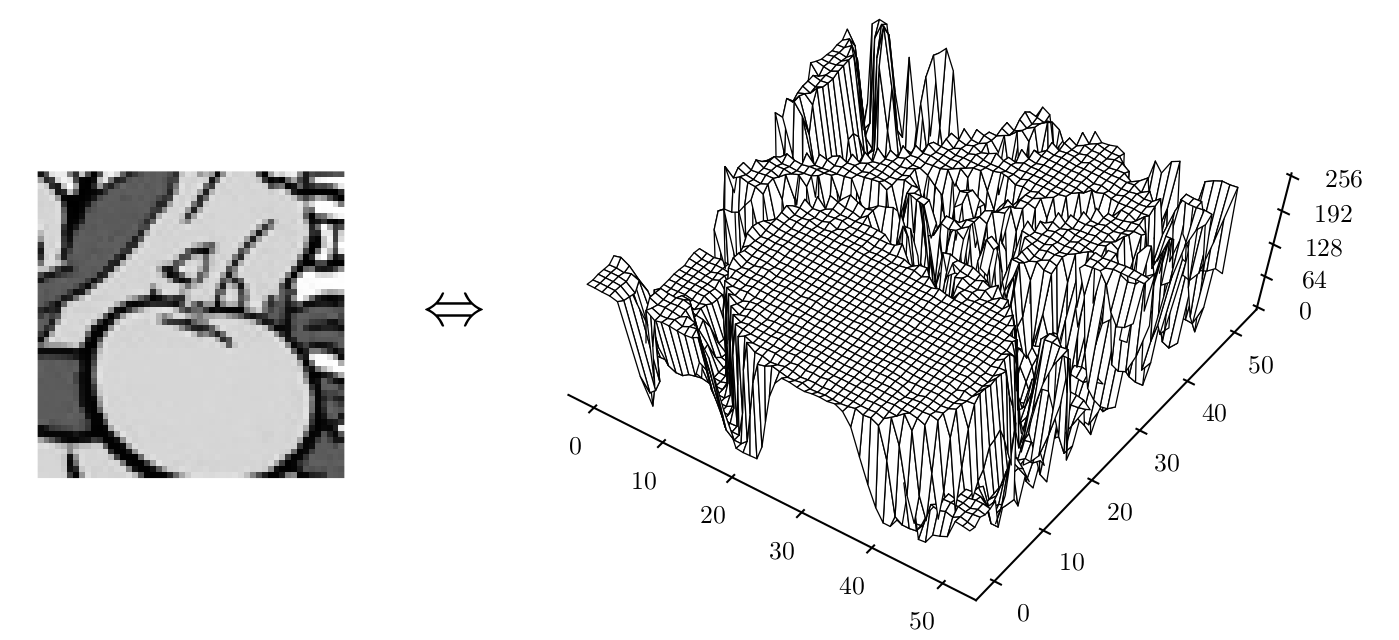
\includegraphics[width=0.9\linewidth]{images/ImageAsAFunctionExample}
	\caption{}
	\label{fig:imageasafunctionexample}
\end{figure}

\underline{Notation}: To signify that $f$ is continuous, write $f(x)$. To signify that $f$ is discrete (partial), write $f[x]$ (with $x\in \{\IR, \IR^2\}$).

\begin{Definition}[Derivatives]{def:Derivatives}
	Let $f$ be a continuous, uni-variate function $f:\IR\to\IR$ where $x\mapsto f(x)$ and $x_0\in \IR$.
	
	At $x_0$, the \textbf{derivative of} $f$ \textbf{from above} is
	\begin{equation} 
		f^\prime_+(x_0) = \lim\limits_{\epsilon\to 0}\frac{f(x_0 + \epsilon) - f(x_0)}{\epsilon} 
	\end{equation}
	At $x_0$, the \textbf{derivative of} $f$ \textbf{from below} is
	\begin{equation} 
		f^\prime_-(x_0) = \lim\limits_{\epsilon\to 0}\frac{f(x_0) - f(x_0-\epsilon)}{\epsilon} 
	\end{equation}
	
	$f$ is \textbf{differentiable} at $x_0$, if
	\begin{equation}
		f^\prime_+(x_0) = f^\prime_-(x_0) = f^\prime(x_0) = \frac{\partial}{\partial x} f(x_0)
	\end{equation}
	In this case, $f^\prime(x_0)$ indicates the \textit{rate of change} of $f$ at $x_0$. That is the \textit{slope of the tangent} of $f$ at $x_0$.
	
	$f$ is differentiable, if it is differentiable at any $x\in\IR$. 
	
	Note that the derivation is a \textbf{linear operator}~\footnote{An \textbf{operator} is a function that maps functions to functions.}:
	\begin{equation}
		\frac{\partial}{\partial x} \Big(af(x) + bg(x) \Big) = a\frac{\partial}{\partial x} f(x) + b\frac{\partial}{\partial x} g(x)
	\end{equation}
\end{Definition}

For the discrete case set for simplicity $x_{i+1} - x_i=1=\epsilon$. Then, the definitions are analogue:\begin{itemize}
	\item \textbf{Backward difference}:
	\begin{equation} 
		f^\prime_-[x] = \frac{f[x]-f[x-1]}{x-(x-1)} = f[x]-f[x-1]
	\end{equation}
	\item \textbf{Forward difference}:
	\begin{equation} 
		f^\prime_+[x] = \frac{f[x+1]-f[x]}{(x+1)-x} = f[x+1]-f[x]
	\end{equation}
	\item \textbf{Central difference}:
	\begin{equation} 
		f^\prime[x] = \frac{f^\prime_+[x]-f^\prime_-[x]}{2} = \frac{f[x+1]-f[x-1]}{2}
	\end{equation}
\end{itemize}

Note that if $f[x]$ has been sampled from $f(x)$, then the central difference of $f[x]$ provides a provably better approximation of the derivative of $f(x)$ than the backward- or forward differences.

Using an operator notation, we will also write the central difference as $f^\prime[x] = d_x f[x]$.

\subsection{Image gradient}

By considering images as functions, we can compute their the gradient. For intensity images $f[x,y]$ it is defined as
\begin{equation}
	\nabla f[x,y] = \begin{bmatrix} d_x f[x,y]\\d_y f[x,y]\end{bmatrix}
	= \frac{1}{2} \begin{bmatrix} f[x+1,y]-f[x-1,y]\\f[x,y+1]-f[x,y-1]\end{bmatrix}
\end{equation}

\begin{figure}[H]
	\centering
	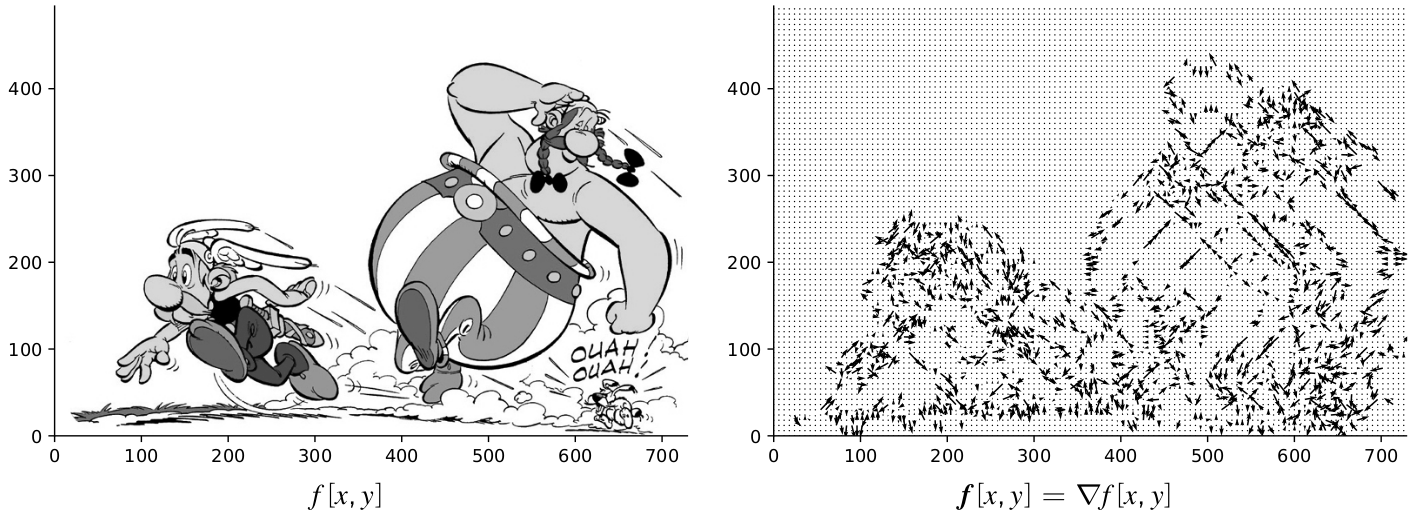
\includegraphics[width=0.9\linewidth]{images/GradientImageExample}
	\caption{Example intensity image and its gradient image.}
	\label{fig:gradientimageexample}
\end{figure}

Gradients of intensity images are typically visualized by only considering its magnitude 
\begin{equation}
	\norm{\nabla f [x,y]} = \sqrt{ \angles{\nabla f[x,y]}{\nabla f[x,y]} }= \sqrt{ \big(\nabla f[x,y]\big)^2 }
\end{equation}

\begin{figure}[H]
	\centering
	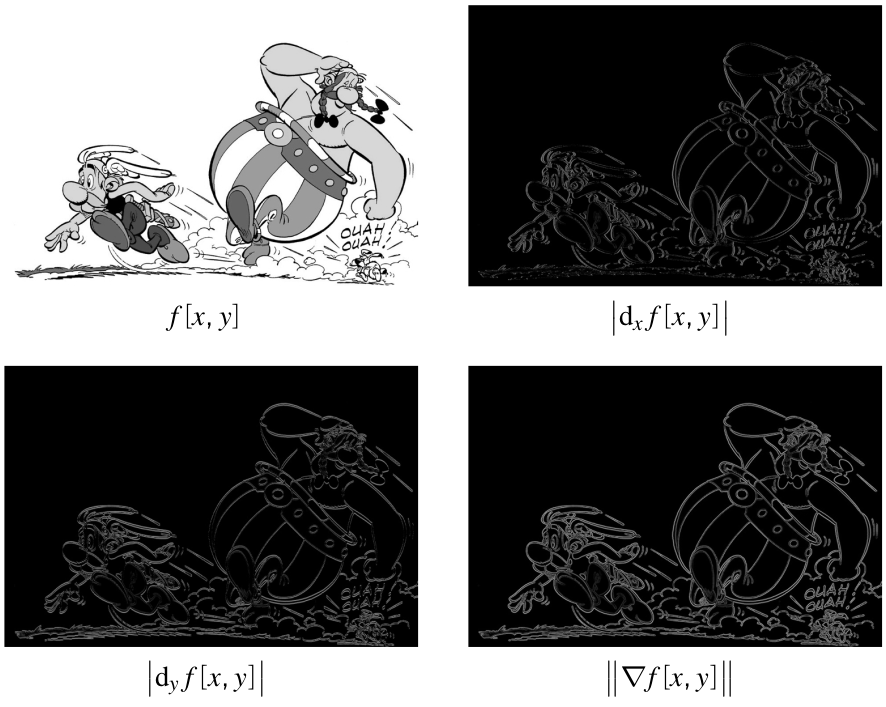
\includegraphics[width=0.7\linewidth]{images/MagnitudeOfGradientsOfIntensityImages}
	\caption{Example of an intensity image, the norms of the directed gradients and the magnitude of the total gradient.}
	\label{fig:magnitudeofgradientsofintensityimages}
\end{figure}

As one can see, the gradient (and its magnitude) can be used as an \textbf{edge detector}.

\subsection{Emboss effect}

The emboss effect transforms an image such that it resembles a copper engraving or an etching. It can be achieved by applying the following operator:
\begin{equation}
	g[x,y] = \max\Big( 0,\ \min\big( 255, \ 128 + f[x+1,y-1] - f[x-1,y+1] \big) \Big)
\end{equation}

Note that by definition it is $0 \le g[x,y] \le 255$. Furthermore, the resulting pixels are computed as $128$ plus the difference in intensity between the lower left and upper right neighboring pixel (diagonal gradient).

\begin{figure}[H]
	\centering
	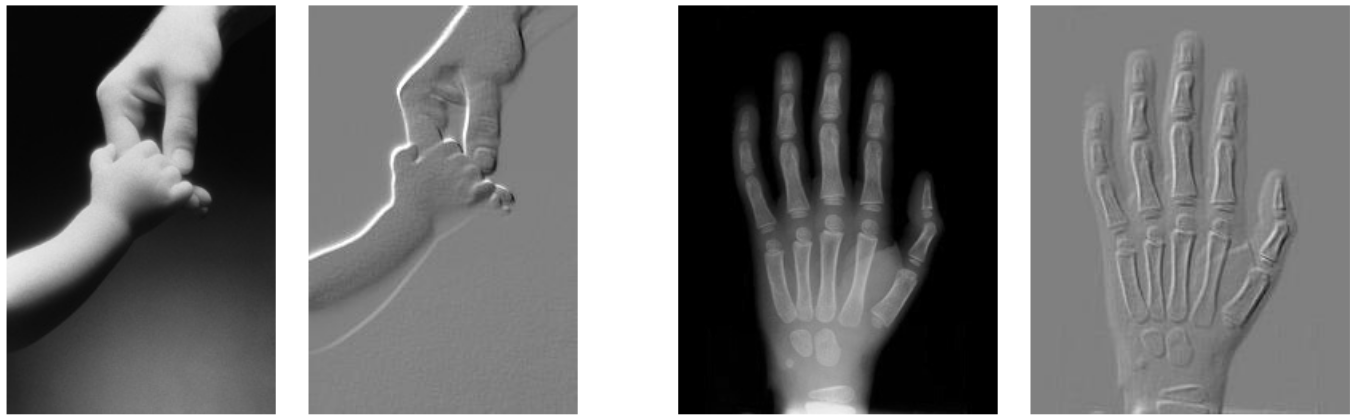
\includegraphics[width=0.9\linewidth]{images/EmbossEffectExamples}
	\caption{Two examples of the emboss effect. Left the original intensity image, right an emboss effect on it.}
	\label{fig:embosseffectexamples}
\end{figure}

%%%%%%%%%%%%%%%%%%%%%%%%%%%%%%%%%%
%%%%% Lecture 04 - 28.20.2021 %%%% - IMPLEMENTATION - notes on C an python
%%%%%%%%%%%%%%%%%%%%%%%%%%%%%%%%%%

%%%%%%%%%%%%%%%%%%%%%%%%%%%%%%%%%%
%%%%% Lecture 05 - 04.11.2021 %%%% - MATH - vector spaces and coordinate systems
%%%%%%%%%%%%%%%%%%%%%%%%%%%%%%%%%%

%%%%%%%%%%%%%%%%%%%%%%%%%%%%%%%%%%
%%%%% Lecture 06 - 08.11.2021 %%%% - MATH - affine coordinate transformations
%%%%%%%%%%%%%%%%%%%%%%%%%%%%%%%%%%

%%%%%%%%%%%%%%%%%%%%%%%%%%%%%%%%%%
%%%%% Lecture 07 - 11.11.2021 %%%% - MATH - polar coordinates and complex exponentials
%%%%%%%%%%%%%%%%%%%%%%%%%%%%%%%%%%

%%%%%%%%%%%%%%%%%%%%%%%%%%%%%%%%%%
%%%%% Lecture 08 - 15.11.2021 %%%% - MATH - a first glance at Fourier transforms
%%%%%%%%%%%%%%%%%%%%%%%%%%%%%%%%%%

%%%%%%%%%%%%%%%%%%%%%%%%%%%%%%%%%%
%%%%% Lecture 09 - 18.11.2021 %%%% - MATH - the Fourier transform
%%%%%%%%%%%%%%%%%%%%%%%%%%%%%%%%%%

%%%%%%%%%%%%%%%%%%%%%%%%%%%%%%%%%%
%%%%% Lecture 10 - tt.mm.2021 %%%% - MATH - properties of the Fourier transform
%%%%%%%%%%%%%%%%%%%%%%%%%%%%%%%%%%

%%%%%%%%%%%%%%%%%%%%%%%%%%%%%%%%%%
%%%%% Lecture 11 - tt.mm.2021 %%%% - MATH - Frequency domain filtering
%%%%%%%%%%%%%%%%%%%%%%%%%%%%%%%%%%

%%%%%%%%%%%%%%%%%%%%%%%%%%%%%%%%%%
%%%%% Lecture 12 - tt.mm.2021 %%%% - MATH - Convolution and FT
%%%%%%%%%%%%%%%%%%%%%%%%%%%%%%%%%%

%%%%%%%%%%%%%%%%%%%%%%%%%%%%%%%%%%
%%%%% Lecture 13 - tt.mm.2021 %%%% - MATH - Convolution and Gaussian filters
%%%%%%%%%%%%%%%%%%%%%%%%%%%%%%%%%%
%\subsection{Gaussian filter} 
%TODO:??? Add to section 'Linear filters'?
%%%%%%%%%%%%%%%%%%%%%%%%%%%%%%%%%%
%%%%% Lecture 14 - tt.mm.2021 %%%% - MATH - FT in terms of bra and ket
%%%%%%%%%%%%%%%%%%%%%%%%%%%%%%%%%%

%%%%%%%%%%%%%%%%%%%%%%%%%%%%%%%%%%
%%%%% Lecture 15 - tt.mm.2021 %%%%
%%%%%%%%%%%%%%%%%%%%%%%%%%%%%%%%%%
\section{Linear filters}

Examples of linear filters are low-pass filters, Gaussian filters and mean filters.\\

\begin{Definition}[Linear filters]{def:LinearFilters}
	Convolution filters 
	\[ h(x)=f(x)*g(x) \]
	(where $f(x)$ is a signal and $g(x)$ is a filter) are called \textbf{convolution filters} because the convolution is a linear operations.
\end{Definition}


\subsection{Gaussian filter}
Space domain image filtering is done by convolution of the image with a filter mask:
\begin{equation*}
	h[x,y] = (f*g)[x,y] = \sum_{u=-\frac{n}{2}}^{\frac{n}{2}} \sum_{v=-\frac{m}{2}}^{\frac{m}{2}} f[x-u,y-v] g[u,v]
\end{equation*}

A 2D convolution with a Gaussian filter mask $G_{\sigma}$ is a separable operation and thus can be computed in terms of two 1D convolutions with two 1D Gaussians. This reduces the per pixel effort from $\mathcal{O}(m^2)$ to $\mathcal{O}(m)$:

\begin{flalign*}
	(f*G_{\sigma})(x,y) &= \frac{1}{2 \pi \sigma^2} \int\limits_{-\infty}^{\infty} \int\limits_{-\infty}^{\infty} f(\xi, v) \exp\Big( -\frac{(x-\xi)^2 + (y-\nu)^2}{2\sigma^2} \Big) d\xi d\nu \\
	&= \frac{1}{2 \pi \sigma^2} \int\limits_{-\infty}^{\infty} \int\limits_{-\infty}^{\infty} f(\xi, v) e^{-\frac{(x-\xi)^2}{2\sigma^2}} e^{\frac{-(y-\nu)^2}{2\sigma^2}} d\xi d\nu \\
	&= \frac{1}{2 \pi \sigma^2} \int\limits_{-\infty}^{\infty} \Big( \frac{1}{\sqrt{2\pi}\sigma} \int\limits_{-\infty}^{\infty} f(\xi, \nu) e^{-\frac{(x-\xi)^2}{2\sigma^2}} d\xi \Big) e^{ \frac{-(y-\nu)^2}{2\sigma^2} } d\nu
\end{flalign*}

\begin{figure}[H]
	\centering
	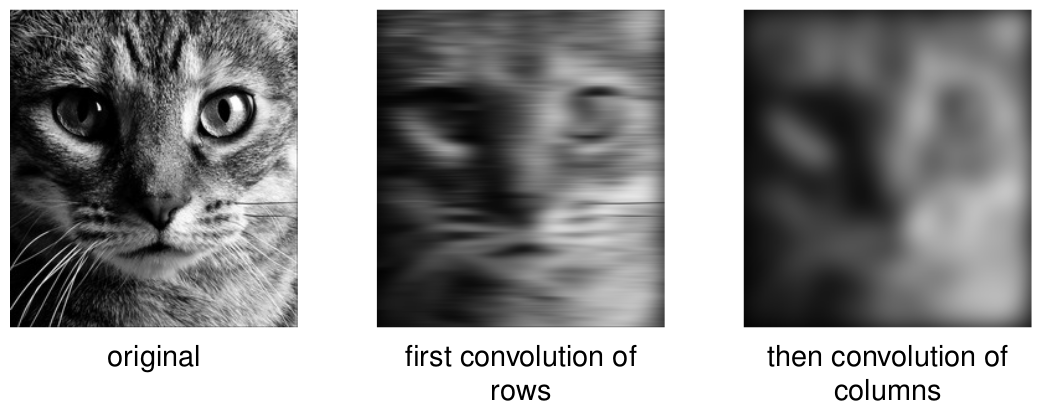
\includegraphics[width=1.0\linewidth]{images/illustration_of_GaussianSeparability}
	\caption{Illustration of the separability of the convolution with a Gaussian filter mask}
	\label{fig:illustrationofgaussianseparability}
\end{figure}

Note that the convolution with a bi-variate Gaussian is separable, because the bi-variate Gaussian itself is separable. For the \textit{continuous}, isotropic case, we have:
\begin{itemize}
	\item Uni-variate Gaussian:
	\[ g_{\sigma}(x) = \frac{1}{\sqrt{2\pi} \sigma} e^{- \frac{x^2}{2\sigma^2}} \]
	\item Bi-variate Gaussian:
	\[ G_{\sigma}(x,y) = \frac{1}{\sqrt{2\pi} \sigma^2} e^{- \frac{x^2+y^2}{2\sigma^2}} = \frac{1}{\sqrt{2\pi} \sigma^2} e^{- \frac{x^2}{2\sigma^2}} e^{- \frac{y^2}{2\sigma^2}} = g_{\sigma}(x)\cdot g_{\sigma}(y)\]
\end{itemize}

For the \textit{discrete}, isotropic case, we have:
\begin{itemize}
	\item Uni-variate Gaussian:
	\[ g_{\sigma}[x_i] = \frac{ e^{- \frac{x_i^2}{2\sigma^2}} }{ \sum_{i} e^{- \frac{x_i^2}{2\sigma^2}} } \]
	\item Bi-variate Gaussian:
	\[ G_{\sigma}[x_i,y_j] = \frac{ e^{- \frac{x_i^2+y_j^2}{2\sigma^2}} }{ \sum_{i, j} e^{- \frac{x_i^2+y_j^2}{2\sigma^2}} }  = g_{\sigma}[x_i] \cdot g_{\sigma}[y_j]\]
\end{itemize}

If we understand the discrete, uni-variate Gaussian as a finite dimensional vector $g\in\IR^m$ with entries
\[ g= \Big[ g_{\sigma}\big[x_{-\frac{m}{2}} \big], \dots, g_{\sigma}[x_0],\dots, g_{\sigma}\big[x_{+\frac{m}{2}} \big] \Big]^\intercal \]
we can think of the discrete, bi-variate Gaussian as a finite dimensional outer product matrix $G\in \IR^{m\times m}$: $G=\opt{g}{g}$.\newline


Note that this also works for non-isotropic yet uncorrelated bi-variate Gaussians:
\[  G_{\sigma_i, \sigma_j}[x_i,y_j] = \frac{ \exp\Big( -\frac{x_i^2}{2\sigma_x^2}-\frac{y_j^2}{2\sigma_y^2} \Big) }{ \sum_{i, j} \exp\Big( -\frac{x_i^2}{2\sigma_x^2}-\frac{y_j^2}{2\sigma_y^2} \Big) }\]

%%%%%%%%%%%%%%%%%%%%%%%%%%%%%%%%%%
%%%%% Lecture 18 - tt.mm.2021 %%%%
%%%%%%%%%%%%%%%%%%%%%%%%%%%%%%%%%%
\subsubsection{Recursive Gaussian filtering}

Since the 2D Gaussian is separable, an efficient 1D Gaussian filter would yield a Gaussian filtering algorithm in $\mathcal{O}(1)$ time. This will be discussed in this section.

Intensity images are discrete bi-variate signals $f[x,y]$. Here, we will focus on discrete uni-variate signals $f[x]$. However, instead of thinking of them as functions of space $x$, we will consider them as functions of time $t$ (to match the terminology used in signal processing).

The key insight is, that a discrete, uni-variate mean filter can be computed \textbf{recursively}:
\begin{flalign*}
	h[t] &= \frac{1}{m} \sum_{i=-\frac{m}{2}}^{\frac{m}{2}} f[t+i]\\
	&= \frac{1}{m} \sum_{i=-\frac{m}{2}}^{\frac{m}{2}-1} f[t+i] + \frac{1}{m} f\big[t+\frac{m}{2}\big]\\
	&= \frac{1}{m} \sum_{i=-\frac{m}{2}-1}^{\frac{m}{2}-1} f[t+i] - \frac{1}{m} f\big[t-\frac{m}{2}-1\big] + \frac{1}{m} f\big[t+\frac{m}{2}\big]\\
	&= \frac{1}{m} \sum_{i=-\frac{m}{2}}^{\frac{m}{2}} f[t-1+i] - \frac{1}{m} f\big[t-1-\frac{m}{2}\big] + \frac{1}{m} f\big[t+\frac{m}{2}\big] \\
	&= h[t-1] - \frac{1}{m} f\big[ t-1-\frac{m}{2} \big] + \frac{1}{m} f\big[ t+\frac{m}{2} \big]
\end{flalign*}

\begin{Definition}[Causal and anti-causal filters]{def:CausalAndAntiCausalFilters}
	Let $f$ be a discrete, uni-variate function and $h$ a filter on it. The \textbf{causal} part of the filter are all terms that only use the past values $f[t-i]$ to compute the filter value at $t$.\\
	The \textbf{anti-causal} part of the filter are all terms that only use the future values $f[t+i]$ to compute the filter value at $t$.
\end{Definition}

Example of causal and anti-causal filter components of mean filtering:
\[ h[t] = \frac{1}{m} \sum_{i=-\frac{m}{2}}^{\frac{m}{2}} f[t+i] =  \underbrace{\frac{1}{m} \sum_{i=0}^{\frac{m}{2}} f[t-i]}_{\text{cuasal}} + \underbrace{\frac{1}{m} \sum_{i=1}^{\frac{m}{2}} f[t+i]}_{\text{anti-cuasal}}\]

In signal processing, the convent is to denote the input to a filter as $x[t]$, and the output of a filter as $y[t]$.

\begin{Definition}[Finite and infinite impulse response filter]{def:FIRandIIRfilters}
	A \textbf{Finite impulse response (FIR) filter} of order $m$ is a causal filter where
	\[ y[t] = a_0 x[t] + a_1 x[t-1] + \dots + a_m x[t-m] \ = \sum_{i=0}^{m} a_i x[t-i] \]
	
	An \textbf{infinite impulse response (IIR) filter} is a causal filter where
	\[ y[t] = \sum_{i=0}^{\infty} a_i x[t-i] \]
\end{Definition}

IIR systems are often modeled in terms of difference equations or \textit{recursive filters}:
\[ y[t] = \sum_{i=0}^{m} a_i x[t-i] - \sum_{i=1}^{n} b_i y[t-i] \]
Lets use the notation
\[ y[n] = \sum_{m=0}^{P} a_m x[n-m] - \sum_{m=1}^{Q} b_m y[n-m] \]
or, equivalently with $b_0=1$
\[ \sum_{m=0}^{Q} b_m y[n-m] = \sum_{m=0}^{P} a_m x[n-m]\]

Such IIR systems have a particularly simple Z-transform or transfer functions. Using $\mathcal{Z}\{ x[n-k] \} = z^{-k} X(z)$ we can write:
\[ Y(z) = \sum_{m=0}^{P} a_m z^{-m}X[z] - \sum_{m=1}^{Q} b_m z^{-m}Y(z) \]
or, again equivalently
\[ Y(z) \Big( 1+\sum_{m=1}^{Q} b_m z^{-m} \Big) = X(z) \sum_{m=0}^{P} a_m z^{-m} \]

Using this we can define a \textit{transfer function}:
\[ H(z) = \frac{Y(z)}{X(z)} = \frac{ \sum\limits_{m=0}^{P}a_m z^{-m} }{ 1+\sum\limits_{m=1}^{Q}b_m z^{-m} }  \]

The transfer function of an IIR system is a rational function (and a ratio of two polynomials). The numerator $Y(z)$ is a convolution, the denominator $X(z)$ is a recursion. The goal is to determine $H(z)$ such that it realizes Gaussian filtering. This consists of two challenges:\begin{enumerate}
	\item Gaussian filtering is only convolutional (that is, there is no recursion). Thus we need to approximate the Z-transform of a Gaussian using two polynomials.
	\item The transfer function is causal (only looks back in time), but Gaussian filtering is anti-causal (requires us to look ahead in time). Thus we need to express an anti-causal filter in terms of causal components only. 
\end{enumerate}

First, lets solve the second challenge. Consider causal and anti-causal components by requiring
\[ h[n] = h_+[n] + h_-[n] \]
where
\[ h_+[n] := \begin{cases}
h[n] & \text{if }n\le 0\\
0 & \text{if } n>0
\end{cases},\qquad h_-[n] := \begin{cases}
0 & \text{if }n\le 0\\
h[n] & \text{if } n>0
\end{cases} \]

We will make use of the following equations (without proofing them):
\begin{equation}\label{eq:ZTransformHPlus}
	\mathcal{Z}\{ h_+[n] \} = H_+(z)= \frac{ \sum_{m=0}^{P-1} a_m^+ z^{-m} }{ 1 + \sum_{m=1}^{Q} b_m^+ z^{-m} }
\end{equation}
\begin{equation}\label{eq:ZTransformHMinus}
	\mathcal{Z}\{ h_-[n] \} = H_-(z)= \frac{ \sum_{m=1}^{P} a_m^- z^{m} }{ 1 + \sum_{m=1}^{Q} b_m^- z^{m} }
\end{equation}
Using these, we construct a recursive Gaussian filter as a sum of a causal- and an anti-causal system $h[n] = h_+[n] + h_-[n]$ or $H(z)=H_+(z) + H_-(z)$.

To implement the composite filter, we apply the causal- and the anti-causal filter to an input sequence $x[n]$ and accumulate their results in an output sequence $y[n]$.\\
It remains to determine the coefficients $a_m^+, b_m^+, a_m^-$ and $b_m^-$. Therefore set $P=Q$. Without proof we claim that\begin{itemize}
	\item for symmetric, even filters, the coefficients are related as
	\begin{flalign*}
		b_m^- &= b_m^+ & && &\forall m\\
		a_m^- &= a_m^+ &- b_m^+ a_0^+ && &\forall m=1,\dots, Q-1\\
		a_Q^- &= &-b_Q^+ a_0^+ &&&&&&&&&&&&&&&&&&&&&&&
	\end{flalign*}
	\item for anti-symmetric, odd filters, we have
	\begin{flalign*}
	b_m^- &= b_m^+ & && &\forall m\\
	a_m^- &= -a_m^+ &+ b_m^+ a_0^+ && &\forall m=1,\dots, Q-1\\
	a_Q^- &= &\; b_Q^+ a_0^+ &&&&&&&&&&&&&&&&&&&&&&&&&&&
 	\end{flalign*}
\end{itemize}
Now only $a_m^+$ and $b_m^+$ have to be determined.\\


The solution to the first challenge, that is to approximate the Z-transform of a Gaussian using two polynomials, goes as follows: Approximate the causal part of 
\[ g_\sigma [n] = \frac{1}{\sqrt{2\pi} \sigma} e^{-\frac{n^2}{2\sigma^2}} \]
as a linear combination of four simple exponential functions
\[ h_\sigma^+[n] = \sum_{i=0}^{k=3} w_i e^{-\lambda_i \frac{n}{\sigma}} \]
because this model has a simple Z-transform. Using substitutions and Euler's identity, we can write
\[ h_\sigma^+[n] = \sum_{i=1}^{2} \Big( \alpha_i \cos\big( \frac{n\omega_i}{\sigma}\big) + \beta_i \sin\big( \frac{n\omega_i}{\sigma} \big) \Big) e^{-\frac{n\gamma_i}{\sigma}} \]

Computing the Z-transform of $h_\sigma^+[n]$ and comparison to $h_+[n]$ in \ref{eq:ZTransformHPlus} yields:
\begin{flalign*}
	a_0^+ = & \; \alpha_1 + \alpha_2 \\
	a_1^+ = & \; e^{-\frac{\gamma_2}{\sigma}} \left( \beta_2 \sin\frac{\omega_2}{\sigma}-(\alpha_2+2 \alpha_1) \cos\frac{\omega_2}{\sigma} \right) + 
	e^{-\frac{\gamma_1}{\sigma}} \left( \beta_1 \sin\frac{\omega_1}{\sigma}-(2 \alpha_2+\alpha_1) \cos\frac{\omega_1}{\sigma} \right) \\
	a_2^+ = & \; 2 e^{-\frac{\gamma_1+\gamma_2}{\sigma}}   
	\left( 
	(\alpha_1+\alpha_2) \cos\frac{\omega_2}{\sigma} \cos\frac{\omega_1}{\sigma}
	- \cos\frac{\omega_2}{\sigma} \beta_1 \sin\frac{\omega_1}{\sigma}
	- \cos\frac{\omega_1}{\sigma} \beta_2 \sin\frac{\omega_2}{\sigma}
	\right) \\
	& \; + \alpha_2 e^{-2 \frac{\gamma_1}{\sigma}} + \alpha_1 e^{-2 \frac{\gamma_2}{\sigma}} \\
	a_3^+ = & \; e^{-\frac{\gamma_2 + 2 \gamma_1}{\sigma}}  \left(\beta_2 \sin\frac{\omega_2}{\sigma}-\alpha_2 \cos\frac{\omega_2}{\sigma}\right)
	+ e^{-\frac{\gamma_1 + 2 \gamma_2}{\sigma}}  \left(\beta_1 \sin\frac{\omega_1}{\sigma}-\alpha_1 \cos\frac{\omega_1}{\sigma}\right) \\
	b_1^+ = & \; -2 e^{-\frac{\gamma_2}{\sigma}} \cos\frac{\omega_2}{\sigma} - 2 e^{-\frac{\gamma_1}{\sigma}} \cos\frac{\omega_1}{\sigma} \\
	b_2^+ = & \; 4 \cos\frac{\omega_2}{\sigma} \cos\frac{\omega_1}{\sigma} e^{-\frac{\gamma_1 + \gamma_2}{\sigma}}
	+ e^{-2 \frac{\gamma_2}{\sigma}} + e^{-2 \frac{\gamma_1}{\sigma}} \\
	b_3^+ = & \; -2 \cos\frac{\omega_1}{\sigma} e^{-\frac{\gamma_1 + 2 \gamma_2}{\sigma}}
	- 2 \cos\frac{\omega_2}{\sigma} e^{-\frac{\gamma_2 + 2 \gamma_1}{\sigma}} \\
	b_4^+ = & \; e^{-\frac{2 \gamma_1 + 2 \gamma_2}{\sigma}}             
\end{flalign*}

To determine the coefficients $\alpha_i$, $\beta_i$, $\omega_i$ and $\gamma_i$, Deriche (1992) resorts to the method of least squares by minimizing the loss function
\[ E=\sum_{n=0}^{1000} \Big[ h_\sigma^+\big[ \frac{n}{100} \big] - g_\sigma \big[ \frac{n}{100} \big] \Big]^2 \]
His results are:
\begin{center}\begin{tabular}{l|c|c|c|c}
	& $\alpha_i$ & $\beta_i$ & $\gamma_i$ & $\omega_i$\\\hline
	$i=1$ & $1.6800$ & $3.7350$ & $1.7830$ & $0.6318$\\
	$i=2$ & $-0.6803$ & $-0.2598$ & $1.7230$ & $1.9970$\\
\end{tabular}\end{center}

Given $\alpha_i, \beta_i, \gamma_i, \omega_i$ and the standard deviation $\sigma$ of the desired Gaussian filter, we can determine $a_m^+, b_m^+, a_m^-$ and $b_m^-$. Using this method to filter a given signal $x[n]$ is then to compute
\[ y[n] = \frac{1}{\sigma\sqrt{2\pi}} \big( y_+[n] + y_-[n] \big)  \]
where
\begin{flalign*}
	y_+[n] &= \sum_{m=0}^{3} a_m^+ x[n-m] - \sum_{m=1}^{4} b_m^+ y^+ [n-m]\\
	y_-[n] &= \sum_{m=1}^{4} a_m^- x[n+m] - \sum_{m=1}^{4} b_m^- y^- [n+m]
\end{flalign*}

In other words, if $x[n]$ is a row (or a column) of an image, we compute e
\begin{itemize}
	\item[] $y_+[n]$ by iterating over $x[n]$ from left to right (top to bottom) and \item[] $y_-[n]$ by iterating over $x[n]$ from right to left (bottom to top).
\end{itemize}
Per pixel, this requires only a fixed number of operations, regardless of our choice of $\sigma$. Thus the computational effort per pixel is $\mathcal{O}(1)$.

An improved (even faster) method for recursive Gaussian filtering can be found in  ~\cite{young1995recursive}.

\subsubsection{Summary}
To summarize, Gaussian filtering can be done with a pixel effort of
\begin{itemize}
	\item $\mathcal{O}(m^2)$ - using naive 2D convolutions and
	\item $\mathcal{O}(m)$ - exploiting separability.
\end{itemize}

\subsection{Mean filter}

\begin{Definition}[Mean filters]{def:MeanFilters}
	A mean filter $g(x)$ can be defined as 
	\[ \frac{1}{mn} \begin{bmatrix} 1 & 1 & \dots & 1\\	
	1 & 1 & \dots & 1\\
	\vdots & \vdots & \ddots & \vdots\\
	1 & 1 & \dots & 1\\
	\end{bmatrix} \]
	Convolution with it assigns every pixel the \textit{average intensity value} of all pixels in its $m\times n$ neighborhood.	
\end{Definition}

Notice that the brute-force effort per pixel of mean filtering is $\mathcal{O}(mn)$. Using intelligent pre-processing, the effort per pixel can be reduced to $\mathcal{O}(1)$!

\subsubsection{Integrals of integrals}

Given an $N\times M$ image $f[x,y]$, we often consider \textbf{integrals}
\[ c[x,y,n,m] = \sum\limits_{u=x-\frac{n}{2}}^{x+\frac{n}{2}} \sum\limits_{v=y-\frac{n}{2}}^{y+\frac{n}{2}} h\Big[ f[u,v] \Big] \]
The function $h$ and thus $c$ may be scalar- or vector-valued.

For the mean filter, we simply have
\[ h\Big[ f[u,v] \Big] = \frac{f[u,v]}{mn} \]

In this setting, it is often beneficial to consider \textbf{integrals of integrals}
\[ C[x,y] = \sum\limits_{u=0}^{x} \sum\limits_{v=0}^{y} c[u,v] \]
where
\[ c[u,v] = c[u, v, 1, 1] = h\Big[ f[u,v] \Big] \]
us computed from only a single pixel.

Although these integrals of integrals necessitate an additional iteration over the image, they can ease computational burden. Because once an integral image $C[x,y]$ is available, its sub-integrals $c[x,y]$ can be computed in constant time.

Consider this:
\begin{flalign*}
	c[x,y,n,m] &= &C\Big[ x+\frac{n}{2}, y+\frac{m}{2} \Big] \\ 
	&&-C\Big[ x+\frac{n}{2}, y-\frac{m}{2} \Big] \\
	&&-C\Big[ x-\frac{n}{2}, y+\frac{m}{2} \Big] \\
	&&+C\Big[ x-\frac{n}{2}, y-\frac{m}{2} \Big] &&& &&& &&& &&& &&& &&& &&& &&&\\
	&=: &\delta+\alpha-\beta-\gamma
\end{flalign*}

\begin{figure}[H]
	\centering
	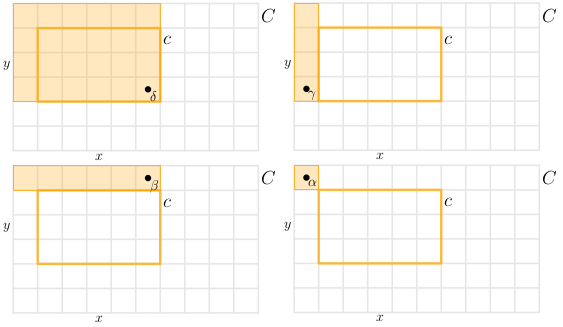
\includegraphics[width=1.0\linewidth]{images/filter_sub_integrals}
	\caption{Illustration of the computation using the sub-integrals.}
	\label{fig:filtersubintegrals}
\end{figure}

The integrals of integrals can be computed efficiently with the following \textit{dynamic program}:
\[ C[x,y] = f[x,y] + C[x,y-1] + C[x-1, y] - C[x-1, y-1] \]

Integral images play a key role in rapid face detection algorithms~\cite{viola2001rapid}. The idea of integral images can be generalized, e.g. to \textit{integral histograms}.\\

\subsubsection{Summary}
To summarize, mean filtering can be done with a pixel effort of
\begin{itemize}
	\item $\mathcal{O}(m^2)$ - using naive 2D convolutions,
	\item $\mathcal{O}(m)$ - exploiting separability and
	\item $\mathcal{O}(1)$ - using integral images.
\end{itemize}

\section{Non-linear filters}


\subsection{Bilateral filter}

Bilateral filtering is a rather recent idea~\cite{tomasi1998bilateral},~\cite{paris2009bilateral}. Given an image $f[x,y]$ and an $n\times m$ neighborhood, compute the new image as
\begin{flalign*}
	h[x,y] &= \gamma[x,y] \sum\limits_{u=-\frac{n}{2}}^{\frac{n}{2}} \sum\limits_{v=-\frac{m}{2}}^{\frac{m}{2}} g_\rho\Big[ f[x,y]-f[x-u,y-v \Big] \cdot G_{\sigma}[u,v]\cdot f[x-u, y-v]\\
	&= \gamma[x,y] \sum\limits_{u=-\frac{n}{2}}^{\frac{n}{2}} \sum\limits_{v=-\frac{m}{2}}^{\frac{m}{2}} H[x,y,u,v]\cdot f[x-u, y-v]
\end{flalign*}
where $g_\rho$ and $G_\sigma$ are Gaussians with standard deviations $\rho$ and $\sigma$ and $\gamma$ is a location dependent normalization factor:
\[ \gamma[x,y] = \frac{1}{ \sum_{u,v} H[x,y,u,v] } \]

\begin{figure}[H]
	\centering
	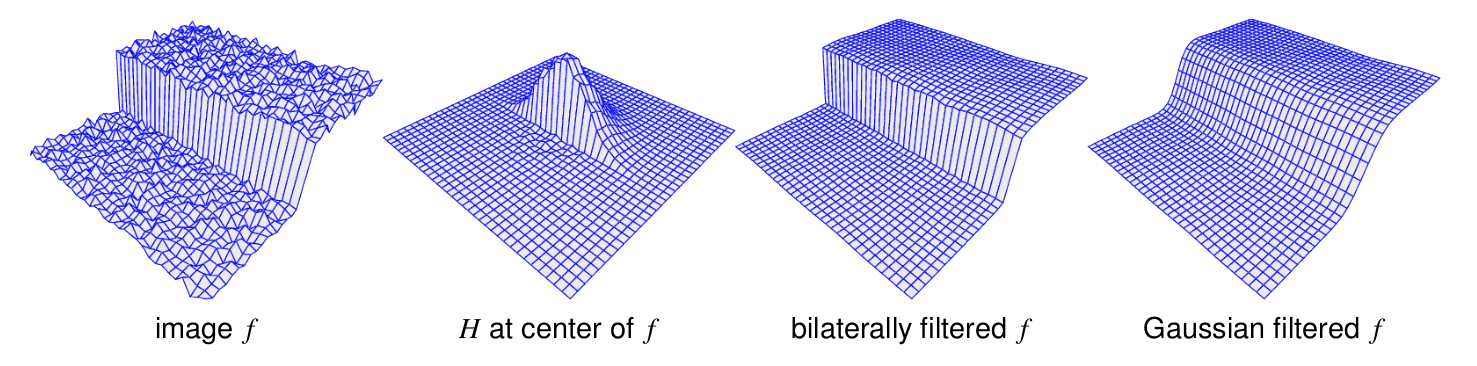
\includegraphics[width=0.7\linewidth]{images/example_bilateral_filtering}
	\caption{Example of bilateral filtering.}
	\label{fig:examplebilateralfiltering}
\end{figure}

%%%%%%%%%%%%%%%%%%%%%%%%%%%%%%%%%%
%%%%% Lecture 16 - tt.mm.2021 %%%%
%%%%%%%%%%%%%%%%%%%%%%%%%%%%%%%%%%
\subsection{Median filter}

Given an 2D image $f$, consider the $m\times n$ neighborhood of pixel $p$ at coordinate $[x,y]$
\[ \mathcal{N}_{xy} := \Big\{ f[i,j]|\ x-\frac{m}{2}\le i \le x+\frac{m}{2} \ \land \  y-\frac{n}{2}\le j \le y+\frac{n}{2} \Big\} := \{ p_0, p_1,\dots, p_{q-1} \} \]
where $q=mn$.

Now, assume that we order the set $\mathcal{N}_{xy}$ ascendingly:
\[ \mathcal{R}_{xy} := \Big\{ r_0, r_1,\dots, r_{q-1}|\ r_i\le r_{i+1}\ \land\ r_i\in\mathcal{N}_{xy} \Big\} \]
Then the element $r_{\frac{q-1}{2}}$ is called the \textbf{median} of the neighborhood $\mathcal{N}_{xy}$.

If we compute the local median for every coordinate $[x,y]$ in $f$ to create a new image $g$, the operation $g[x,y]\leftarrow r_{\frac{q-1}{2}}$ is called \textbf{median filtering}.

\begin{figure}[H]
	\centering
	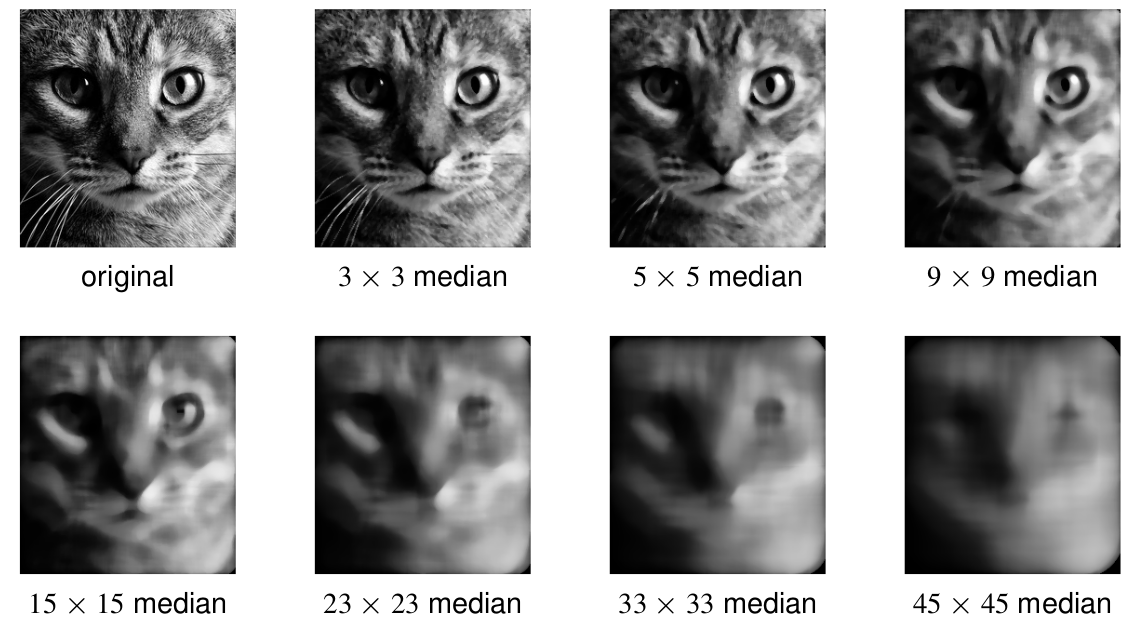
\includegraphics[width=0.7\linewidth]{images/example_median_filtering}
	\caption{Example of median filtering with different sizes of neighborhoods.}
	\label{fig:examplemedianfiltering}
\end{figure}


\begin{algorithm}[H]
	\caption{Naive Median filtering} \label{alg:NaiveMedianFiltering} 
	\begin{tabbing}
		\textbf{Output:} \= \kill
		\textbf{Input:} \>an image $f$ of size $M\times N$,\\
		\>Filter dimensions $m$ and $n$ (size of the considered pixel neighborhood).\\
		\textbf{Output:} \>the median filtered image $g$ of $f$.
	\end{tabbing}	
	\begin{algorithmic}[1]		
		\For {$y=\frac{m}{2}, \dots, M-\frac{m}{2}$}
			\For {$y=\frac{n}{2}, \dots, N-\frac{n}{2}$}
				\State $\mathcal{N}_{xy} = \emptyset$
				\For {$j=-\frac{m}{2}, \dots, \frac{m}{2}$}
					\For {$i=-\frac{n}{2}, \dots, \frac{n}{2}$}
						\State $\mathcal{N}_{xy} = \mathcal{N}_{xy}\cup \Big\{ f[y+i,x+i]\Big\}$
					\EndFor
				\EndFor
				\State $\mathcal{R}_{xy} = \operatorname{qsort}(\mathcal{N}_{xy})$
				\State $g[y,x] \leftarrow r_{\frac{q-1}{2}}$
			\EndFor
		\EndFor
	\end{algorithmic}
	\textbf{Runtime}: Notice that the neighborhoods at the borders of the image are smaller. The average effort per pixel is $\mathcal{O}\big(mn\log(mn)\big)$. If $mn$ is large, this is rather slow.
\end{algorithm}

A more efficient computation can make use of the fact, that the median is the $0.5$ quantile of a given distribution. A histogram $H[i]$ is used to count objects, for example the number of occurrences of an intensity $i$ in an image. When normalized such that its entries sum to $1$, a histogram becomes a \textit{probability mass function}.

\begin{algorithm}[H]
	\caption{Huang Median filtering, 1979} \label{alg:HuangMedianFiltering} 
	\begin{tabbing}
		\textbf{Output:} \= \kill
		\textbf{Input:} \>an image $f$ of size $M\times N$,\\
		\>Filter dimensions $m$ and $n$ (size of the considered pixel neighborhood).\\
		\textbf{Output:} \>the median filtered image $g$ of $f$.
	\end{tabbing}	
	\begin{algorithmic}[1]		
		\For {$y=\frac{m}{2}, \dots, M-\frac{m}{2}$}
			\For {$y=\frac{n}{2}, \dots, N-\frac{n}{2}$}
				\If {$[y,x]$ is in the upper left corner}
					\State Initialize histogram $H$
				\Else
					\For{$k=-\frac{m}{2},\dots, \frac{m}{2}$}
						\State Subtract $f[y+k, x-\frac{n}{2}-1]$ from $H$
						\State Add $f[y+k, x+\frac{n}{2}]$ to $H$
					\EndFor
				\EndIf
				\State $q=\sum_{i} H[i]$
				\State $s=0$
				\For {$i=0,\dots,\#\text{colors}$}
					\State $s=s+H[i]$
					\If {$s\ge \frac{q}{2}$}
						\State $\text{median} = i$
						\State \textbf{break}
					\EndIf
				\EndFor
			\EndFor
		\EndFor
	\end{algorithmic}
	\textbf{Runtime}: The effort per pixel is limited by the number of colors (available intensity values). For an 8-bit gray scale image it is:
	\[ \mathcal{O}(n) + 256\text{ operations} = \mathcal{O}(n) + \mathcal{O}(1) = \mathcal{n}\] 
\end{algorithm}

\begin{figure}[H]
	\centering
	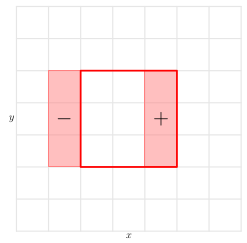
\includegraphics[width=0.7\linewidth]{images/Huang_Alg_Sketch}
	\caption{Sketch of the operations in the Huang median filter (algorithm \ref{alg:HuangMedianFiltering}).}
	\label{fig:huangalgsketch}
\end{figure}

Furthermore we can make use of the fact, that the histogram of disjoint sets is the sum of their individual histograms:
\[ \forall A, B:\qquad A\cap B=\emptyset \ \implies \ H[A\cup B] = H[A] + H[B] \]

Thus one may maintain a histogram $h_x$ for each column $x$ of $f$. This leads to the following algorithm:

\begin{algorithm}[H]
	\caption{Perreault \& H�bert Median filtering, 2007} \label{alg:PerreaultHebertMedianFiltering} 
	\begin{tabbing}
		\textbf{Output:} \= \kill
		\textbf{Input:} \>an image $f$ of size $M\times N$,\\
		\>Filter dimensions $m$ and $n$ (size of the considered pixel neighborhood).\\
		\textbf{Output:} \>the median filtered image $g$ of $f$.
	\end{tabbing}	
	\begin{algorithmic}[1]		
		\For {$y=\frac{m}{2}, \dots, M-\frac{m}{2}$}
			\For {$y=\frac{n}{2}, \dots, N-\frac{n}{2}$}
				\If {$y$ is in the uppermost row}
					\State Initialize a histogram $h_x$ for the column $x$
				\EndIf
				\If {$[y,x]$ is in the upper left corner}
					\State Initialize $H$
				\Else
					\State Subtract $f[y-\frac{m}{2}-1, x+\frac{n}{2}]$ from $h_{x+\frac{n}{2}}$
					\State Add $f[y+\frac{m}{2}, x+\frac{n}{2}]$ to $h_{x+\frac{n}{2}}$
					\State $H=H-h_{x-\frac{n}{2}-1} + h_{x+\frac{n}{2}}$
				\EndIf
				\State $s=0$
				\For {$i=0,\dots,\#\text{colors}$}
					\State $s=s+H[i]$
					\If {$s\ge \frac{q}{2}$}
						\State $\text{median} = i$
						\State \textbf{break}
					\EndIf
				\EndFor
			\EndFor
		\EndFor
	\end{algorithmic}
	\textbf{Runtime}: The effort per pixel is limited by the number of colors (available intensity values). For an 8-bit gray scale image it is:
	\begin{itemize}
		\item One addition and one subtraction for $h_{x+\frac{n}{2}}$
		\item $256$ additions and $256$ subtractions for $H=H-h_{x-\frac{n}{2}-1}+h_{x+\frac{n}{2}}$
		\item At most $256$ operations for computing $s$.
	\end{itemize}
	Thus the runtime is of constant complexity: $\mathcal{O}(1)$. \\
	However note, that there is a large constant factor. Yet, additional tricks keep the efforts low, e.g. multilevel histograms and additions and subtraction by means of bit shifting.
\end{algorithm}

A corresponding implementation is available with OpenCV.

\begin{figure}[H]
	\centering
	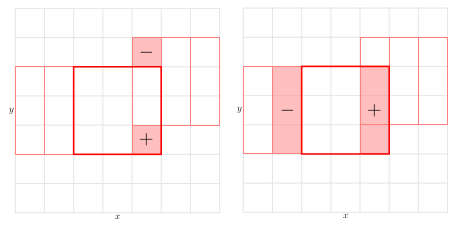
\includegraphics[width=0.7\linewidth]{images/perreault_hebert_mean_filter_sktech}
	\caption{Sketch of the operations in the Perreault \& H�bert median filter (algorithm \ref{alg:PerreaultHebertMedianFiltering}).}
	\label{fig:perreaulthebertmeanfiltersktech}
\end{figure}

To summarize, mean filtering can be done with a pixel effort of
\begin{itemize}
	\item $\mathcal{O}\big(m^2 \log(m^2)\big)$ - using naive 2D convolutions (with qsort),
	\item $\mathcal{O}(m)$ - using local histogram updates and
	\item $\mathcal{O}(1)$ - using clever histogram updates.
\end{itemize}

\section{Morphological operations}

\begin{Definition}[Erosion and dilation]{def:ErosionAndDilation}
	Given $f[x,y]$ and an ordered set $\mathcal{R}_{xy} = \{ r_i\in\mathcal{N}_{xy}| \ r_i\le r_{i+1} \}$, the operation
	\begin{itemize}
		\item $e:g[x,y] \leftarrow r_0$ is called \textbf{erosion} (spread of small values) and
		\item $d:g[x,y] \leftarrow r_{q-1}$ is called \textbf{dialation} (spread of large values).
	\end{itemize}
\end{Definition}

Erosion and dilation are useful in binary image processing. They shrink (erosion) or expand (dilation) shapes. This can also be useful to extract the boundary of a shape. See image \ref{fig:catexampleerosiondilation} for example.

\begin{figure}[h]
	\centering
	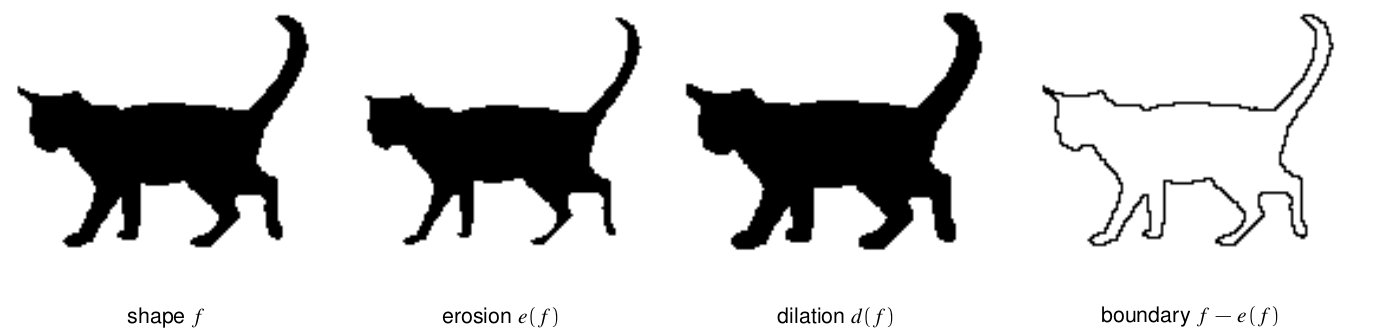
\includegraphics[width=0.7\linewidth]{images/cat_example_erosion_dilation}
	\caption{Example of erosion and dilation on a binary image of the shape of a cat.}
	\label{fig:catexampleerosiondilation}
\end{figure}

\begin{Definition}[Opening and closing]{def:OpeningAndClosing}
	Given $f[x,y]$ and an ordered set $\mathcal{R}_{xy} = \{ r_i\in\mathcal{N}_{xy}| \ r_i\le r_{i+1} \}$. Using erosion $e$ and dialation $d$ one can define the operations
	\begin{itemize}
		\item \textbf{opening} $d \circ e$ and
		\item \textbf{closing} $e \circ d$.
	\end{itemize}
\end{Definition}

\begin{figure}[H]
	\centering
	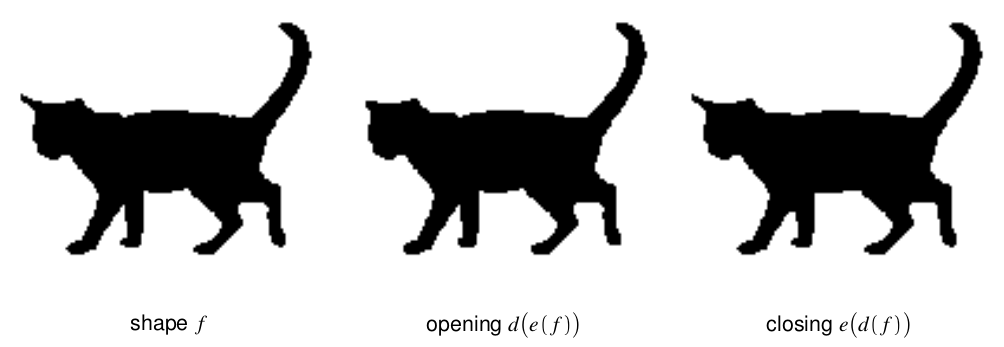
\includegraphics[width=0.7\linewidth]{images/catExampleOpeningAndClosing}
	\caption{Example of the opening and closing operation on a binary image of the shape of a cat.}
	\label{fig:catexampleopeningandclosing}
\end{figure}

Morphological operations are important in areas such as industrial computer vision (machine vision) and in medical image processing. See ~\cite{gonzalez2009digital} and ~\cite{jahne2005applications} for more details.


%%%%%%%%%%%%%%%%%%%%%%%%%%%%%%%%%%
%%%%% Lecture 19 - tt.mm.2021 %%%% - Omitted - due to lack of clear structure
%%%%%%%%%%%%%%%%%%%%%%%%%%%%%%%%%%




\chapter{GOTO END}
\newpage
%%%% ----------------------- %%%%
%%%% -------Exercises------- %%%%
%%%% ----------------------- %%%%

% !TeX spellcheck = en_GB 

\chapter{Exercises}
\section{Sheet 0 - Questions in the lecture slides}

\subsection{Q1 - lecture 02} 
Assume you have an RGB image of resolution $1024\times 768$ with $256$ intensity levels per color channel. How many bytes of memory does such an image require when loaded into a computer?
\paragraph{Solution:} 
To store $256=2^8$ intensity levels exactly eight bits (one byte) is required. Thus to store $1024\times 768 = 786,432$ pixels (intensity levels), \num[group-separator={,}]{786432} bytes are required.

\newpage
\section{Sheet 1}

\subsection{Assignment 1a - Bias of an estimator} 
\dots
\paragraph{Solution:} 



%%%% ----------------------- %%%%
%%%% ------Bibliography----- %%%%
%%%% ----------------------- %%%%
\newpage
\printbibliography

\end{document}
